\section{Rede Neural}

O termo mais apropriado é rede neural artificial, já que apenas rede
neural pode se referir ao sistema biológico de nervos, no antando dado o
contexto desse texto e o uso consagrado do termo ``rede neural'', esse
será usado no lugar da versão mais explícita ``rede neural artificial''.

Uma rede neural é um sistema inspirado no sistema nervoso central (em
especial o cérebro) encontrado em muitos animais. A ideia básica é ter
um grafo em que cada nó abstrai um neurônio e é representado como uma
função, alguns desses nós são responsáveis pela observação e outros pela
saída e os nós de entrada alimentam os próximos nós até chegar nos nós
de saída. \cite{haykin2001redes}

% referencia para "citar" imagens http://www.latex-community.org/forum/viewtopic.php?f=50&t=9115

% TODO melhorar figuras, explicar sigmoid

\begin{figure}[ht]
\centering
%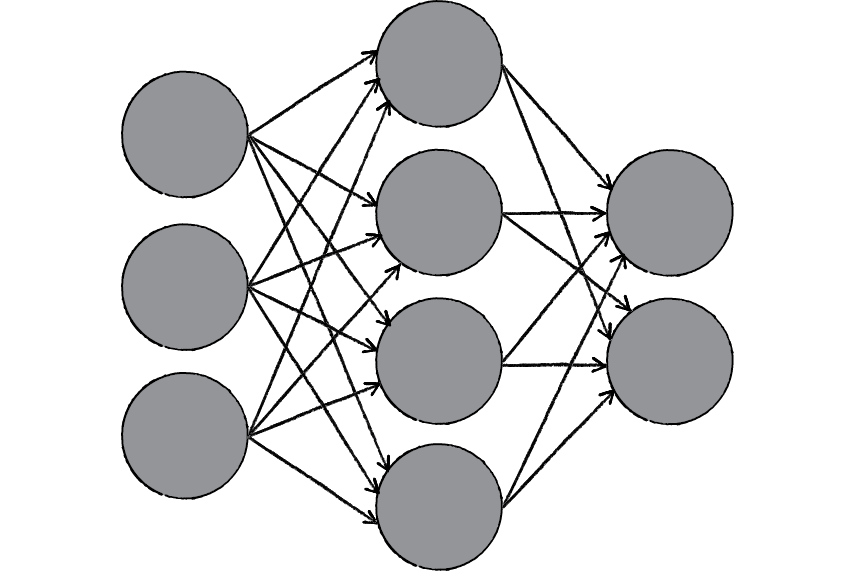
\includegraphics[width=10cm]{figuras/rede_neural_grafo}
%\caption{Rede neural com três camadas.}\label{fig:rede_neural_grafo}
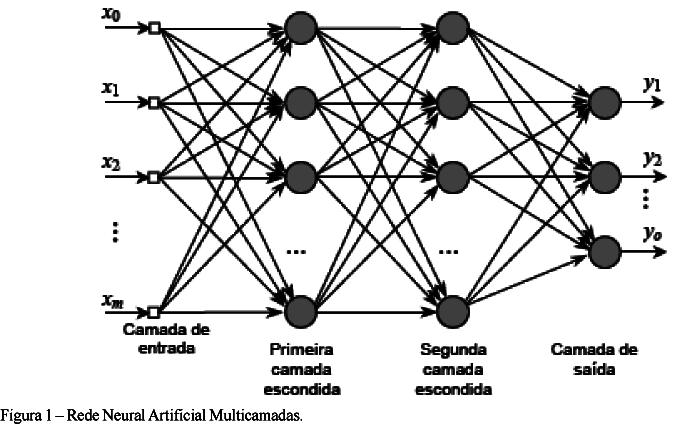
\includegraphics[width=9cm]{figuras/rede_neural_topologia}
\caption{Rede neural com duas camadas ocultas.}\label{fig:rede_neural_grafo}
\end{figure}

A figura~\ref{fig:rede_neural_grafo} exemplifica uma rede neural \emph{feedforward},
que é baseada num grafo direcionado acíclico, em que podem ser vistas 3 camadas
a primeira é chamada de camada de entrada, a última, de saída e as intermediárias,
de escondidas. \cite{shiffman2012nature}

% XXX: desnecessário:
%Um dos diferencias da rede neural é a capacidade de aprender, essa heurística
%forma um sistema adaptativo. Existem três tipos de aprendizados:
%
%\begin{itemize}
%\item
%  Aprendizado supervisionado: alimentar a rede com um problema cuja a solução é conhecida
%  e depois fornecer a resposta certa para que a rede possa se ajustar.
%\item
%  Aprendizado não supervisionado: consiste em buscar padrões não conhecidos, não se conhece
%  a resposta certa ou se uma resposta é certa ou não.
%\item
%  Aprendizado por reforço: alimentar a rede com um problema cuja a solução pode ser avaliada
%  em boa ou má. Esse tipo de aprendizado é comum em robótica onde o robô caminha por um ambiente
%  e tem o reforço negativo ou positivo de colidir ou encontrar o objetivo.
%\end{itemize}

\subsection{O \textit{Perceptron}}

O bloco de construção básico de uma rede neural são os neurônios. Um \textit{perceptron} é a rede
neural mais simples possível: é formada por apenas um neurônio.

\begin{figure}[ht]
\centering
%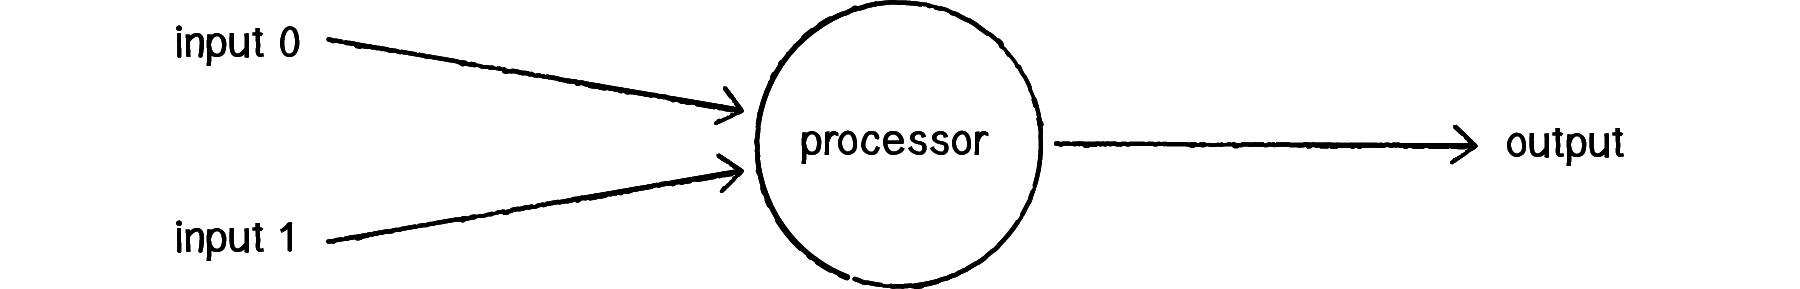
\includegraphics[width=15cm]{figuras/rede_neural_perceptron}
%\caption{\textit{Perceptron} de duas entradas e uma saída.}\label{fig:rede_neural_perceptron}
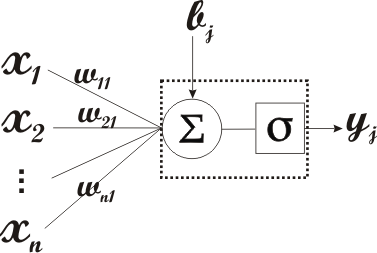
\includegraphics[width=7cm]{figuras/rede_neural_neuronio}
\caption{\textit{Perceptron} de duas entradas e uma saída.}\label{fig:rede_neural_perceptron}
\end{figure}

%A figura~\ref{fig:rede_neural_perceptron} mostra um perceptron com neurônio.

O funcionamento de um \textit{perceptron} pode ser descrito nos seguintes passos:

\begin{itemize}
\item
  Receber e armazenar as entradas;
\item
  Pesar as valores armazenados: consiste em multiplicar cada um pelo peso correspondente àquela entrada;
\item
  Aplicar a função de ativação na soma calculada e armazenar o resultado;
\item
  Enviar o resultado armazenado para a saída.
\end{itemize}

A função de ativação é especialmente útil para resolução de problemas não
lineares. Para problemas cuja a solução é binária se utiliza a função degrau
(ou de Heavside) para discretizar a saída em 2 valores. Outra função de
ativação muito comum é a \textit{sigmoid}, que se aproxima bastante da curva de
aprendizado natural biológica.

\subsection{Exemplo de Aplicação}

Considere uma reta em $\Re^2$, que separa o plano em duas regiões $A$ e $B$. O problema a
ser resolvido pelo \textit{perceptron} é dizer se um ponto $(x,y)$ está em $A$ ou $B$. As entradas do
problema são as coordenadas $x$ e $y$, e a saída é um escalar cujo o valor é um escalar positivo
para sinalizar o conjunto $A$ e negativo para sinalizar o $B$.

O \textit{perceptron} poderia ser modelado com duas entradas, porém note que desse modo o
ponto $(0,0)$ sempre irá resultar numa saída igual a $0$. Para evitar isso são usadas três entradas
no \textit{perceptron} sendo que uma delas é sempre igual a $1$ e é chamada de \emph{bias}, que serve
basicamente para adicionar um peso aditivo e não só multiplicativo. O funcionamento desse \textit{perceptron}
ser observado na figura~\ref{fig:rede_neural_simple_problem}.

\begin{figure}[ht]
\centering
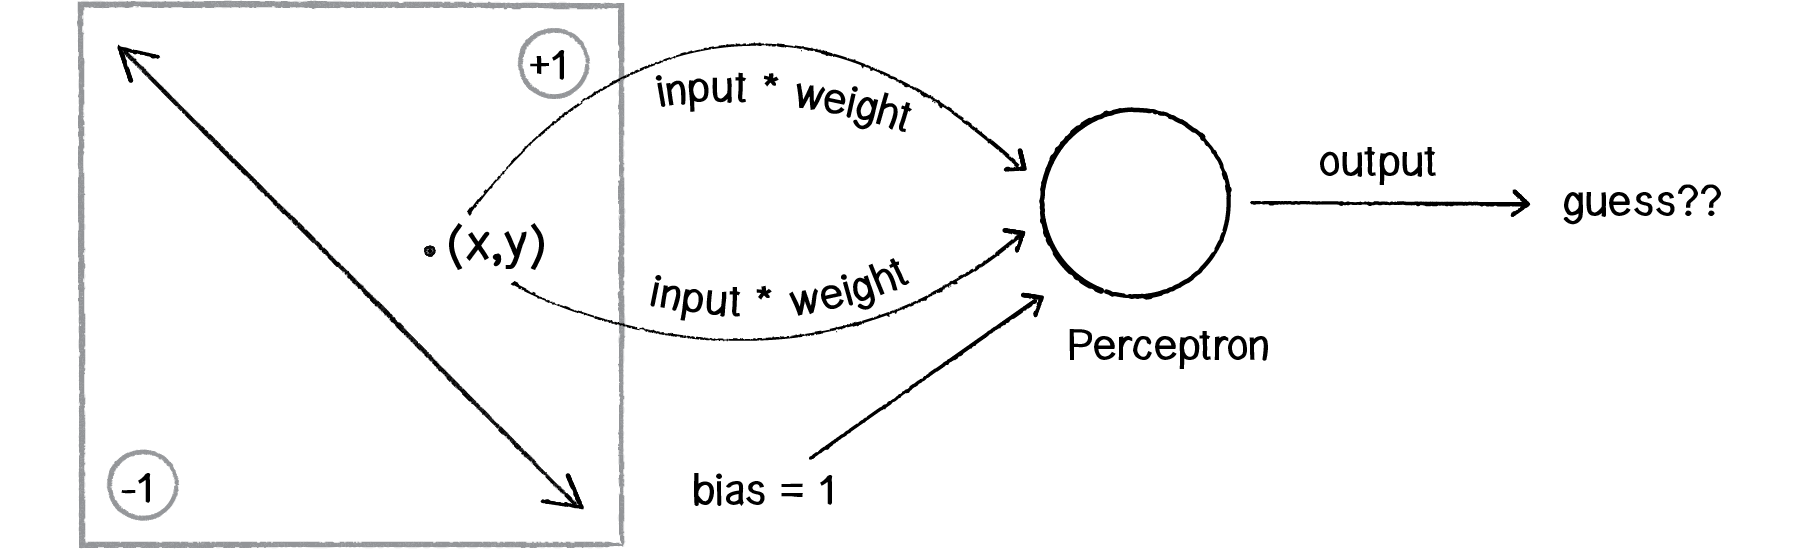
\includegraphics[width=15cm]{figuras/rede_neural_simple_problem}
\caption{\textit{Perceptron} para decidir região de um ponto no plano.}\label{fig:rede_neural_simple_problem}
\end{figure}

Esse exemplo usará o método supervisionado de aprendizado, que funciona da seguinte maneira:

\begin{itemize}
\item
  Alimentar o \textit{perceptron} com uma entrada para o qual se conhece a resposta;
\item
  Pedir a saída ao \textit{perceptron};
\item
  Computar o erro;
\item
  Ajustar os pesos de acordo com o erro;
\item
  Repetir o processo.
\end{itemize}

O ajuste dos pesos pode ser feito calculando o erro e incrementando o peso um fator de
aprendizado vezes o erro vezes a entrada daquele peso.

Assim o \textit{perceptron} é capaz de ser treinado e sua saída ser cada vez mais próxima da desejada.

%\ldots{}

%\begin{itemize}
%\itemsep1pt\parskip0pt\parsep0pt
%\item
%  http://en.wikipedia.org/wiki/Neural\_network
%\item
%  http://en.wikipedia.org/wiki/Artificial\_neural\_network
%\item
%  HAYKIN, S. Redes neurais princípios e prática.
%\end{itemize}


\subsection{Aplicação ao problema}

No contexto do problema proposto uma rede neural poderia ser utilizada em duas vertentes.
A primeira, e mais simples, é na otimização genérica de funções eventuais.
A segunda, e mais complexa, é na detecção de padrões.
O diferencial dessa técnica é a detecção de padrões, por isso a segunda vertente é mais apropriada.
% TODO o Maj Duarte: muito vago

Concretizando melhor a aplicação os cenários mais provável é alimentar uma rede neural
com os dados de estado do jogo e treiná-la para identificar padrões do time inimigo.
Mais formalmente isso se traduz a classificar os estados do jogo em relação ao subconjunto de
informações desse estado associado ao time inimigo.

% TODO Algoritimos de treinamente
% TODO ~Adline~
% TODO Backpropagation
